\section{Experiments}
\label{sec:experiments}

\subsection{Questions, Comparators, and Reporting Rules}

The experiments answer four separate questions. First, does proxy-supervised representation adjustment reduce ATE error relative to adjustment using $X$ alone? Second, do the exact-assumption designs recover the known balancing structure? Third, does the finite-state experiment verify the established certificate and its failure as the proxy channel becomes ill-posed? Fourth, does the method show a useful descriptive signal in an observational benchmark with a noisy randomized reference? We report mean absolute error, root mean squared error, paired wins, held-out discrepancy, overlap diagnostics, and Monte Carlo uncertainty. Oracle procedures that observe $U$ or the true balancing score are simulation references, not implementable competitors.

\subsection{Honest Approximate SCMs}

The primary approximate study fixes the causal order $U\to(X,W)$, $(X,U)\to A$, and $(A,X,U)\to Y$. Both SCMs use $\dim(X)=20$ and $\dim(W)=10$, with twenty independently generated data sets and nested prefixes $n\in\{100,200,500,1000,2000,5000,10000\}$. SCM1 uses linear proxy measurements and a nonlinear outcome component; SCM2 changes the structural equations to nonlinear transformations while preserving the same causal order and an informative monotone proxy channel. The proposed cross-mask method learns a representation from $X$ and all but one proxy coordinate, audits balance with the held-out coordinate, and averages over masks.

At $n=1000$, the mean absolute errors of proposed/$X$-adjustment/full-$(X,W)$/oracle-$(X,U)$ were $0.169/0.601/0.310/0.130$ in SCM1 and $0.112/0.440/0.188/0.107$ in SCM2. At $n=10000$, the corresponding proposed errors were $0.199$ and $0.134$, versus $0.588$ and $0.413$ for $X$ adjustment. These are finite-sample simulation results, not a proof of the audit-view identification theorem. The self-conditioned heuristic remained substantially biased, which is consistent with the self-conditioning warning in Section~\ref{sec:identification}.

\begin{figure}[t]
\centering
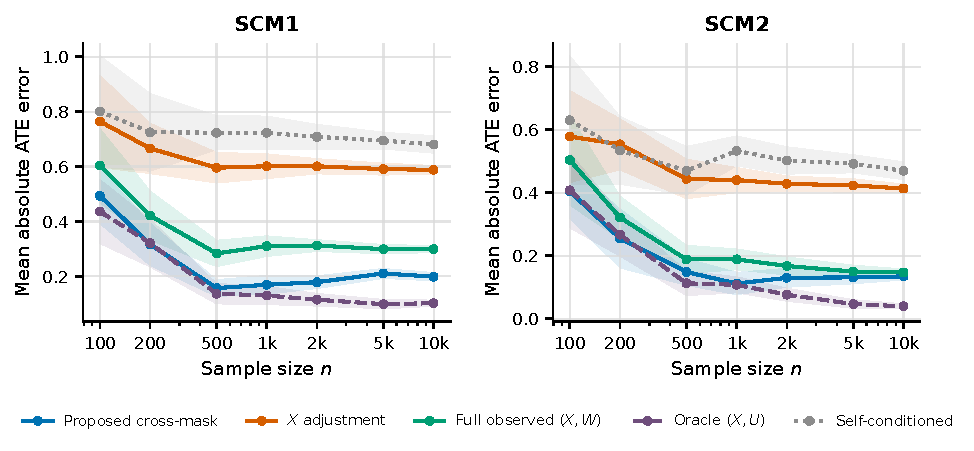
\includegraphics[width=\linewidth]{../figures/final/figure_approximate_scms.pdf}
\caption{Honest approximate SCMs. Curves show mean absolute ATE error across twenty independently generated data sets; bands are approximate $95\%$ Monte Carlo intervals for the mean. Prefixes are nested within a data set, so uncertainty is computed separately at each $n$ and is not pooled across sample sizes. The proposed cross-mask learner uses one proxy coordinate for held-out auditing and averages across masks.}
\label{fig:approximate-scms}
\end{figure}
\FloatBarrier

\subsection{Exact-Assumption Tracks A and B}

Track A uses a finite balancing score, $\dim(X)=20$, nine representation-side proxy coordinates, and one independent audit coordinate. The DGP enforces strict population overlap, exact decoding of the discrete confounding state from the representation-side view, and an injective Gaussian audit channel. At $n=10000$ over twenty replications, mean absolute error was $0.175$ for the learned audit representation, $0.433$ for $X$ adjustment, $0.186$ for direct full-observed adjustment, and $0.033$ for the oracle balancing score. The primary comparison with $X$ passed, while the prespecified secondary superiority criterion against full-observed adjustment failed.

Track B uses a continuous exact balancing score and a linear representation class matched to that score. At $n=10000$, mean absolute error was $0.0748$ for the learned representation, $0.1583$ for fitted $X$ adjustment, and $0.1342$ for fitted full-observed adjustment. The learned method beat $X$ in $20/20$ and full-observed adjustment in $19/20$ paired replications. Its mean rank-recovery Spearman correlation was $0.915$. The held-out conditional-dependence diagnostic used finite random features and is a surrogate, not an exact population KCI test; the design also covers one prespecified scalar-$U$ SCM family.

\begin{figure}[t]
\centering
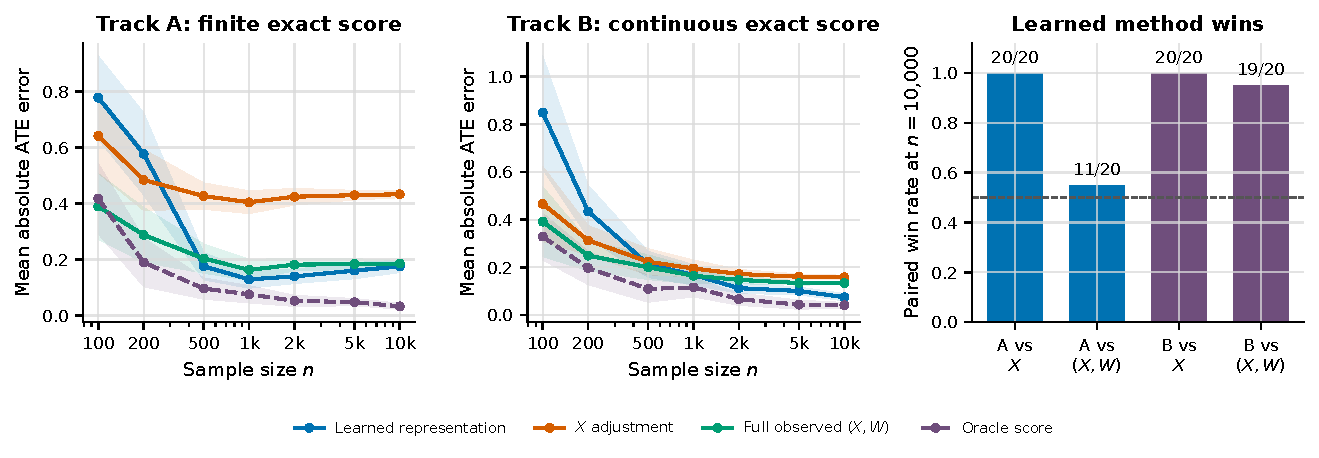
\includegraphics[width=\linewidth]{../figures/final/figure_exact_tracks.pdf}
\caption{Exact-assumption experiments. The first two panels report mean absolute ATE error with approximate $95\%$ Monte Carlo intervals over twenty replications. The third panel reports paired win rates at $n=10{,}000$, where a win means that the learned representation has smaller absolute error than the indicated comparator. Track A satisfies the primary comparison with $X$ but not the prespecified secondary superiority criterion against full observed adjustment. Track B records rank-recovery Spearman correlation $0.915$ and held-out finite-RFF conditional-dependence surrogate $0.00691$.}
\label{fig:exact-tracks}
\end{figure}
\FloatBarrier

\subsection{Finite-State Verification of the Certificate}

The population verification enumerates all $3^{10}$ candidate maps, of which $55{,}980$ satisfy the admissibility conditions. Exactly $3!=6$ maps attain exact balance, and their biases are zero to machine precision. The common certificate has zero violations over all admissible maps. As the proxy channel approaches non-injectivity, the relevant stability constant grows from $1.64$ to $48.9$ and then diverges, even while the observable discrepancy can shrink. This is the intended sensitivity behavior: a small discrepancy is informative only together with a credible stability budget. The explicit finite-sample radius is valid but conservative in this design.

\subsection{WSC Observational Benchmark}

The WSC study forms an observational subset of $1{,}105$ participants whose randomized mathematics assignment agrees with pretreatment preference, and targets the population ATE in the original $2{,}200$ randomized participants. The full randomized difference in means is $0.760$ with standard error $0.151$ and serves only as a noisy benchmark. Across ten algorithmic split repetitions on this one fixed data set, the unconstrained cross-mask estimate averaged $1.302$ with split standard deviation $0.065$ and absolute benchmark gap $0.541$, compared with gaps $2.690$ for the naive observational contrast, $1.704$ for direct $X$ adjustment, and $0.672$ for direct $(X,W)$ adjustment. The unconstrained cross-mask method is the proposed WSC method shown in Figure~\ref{fig:certificate-wsc}. Its practical-overlap gate passed $0/10$ repetitions. The benchmark therefore supplies descriptive evidence only, not a validated causal-performance claim, causal ground truth, or a test of proxy validity.

\begin{figure}[t]
\centering
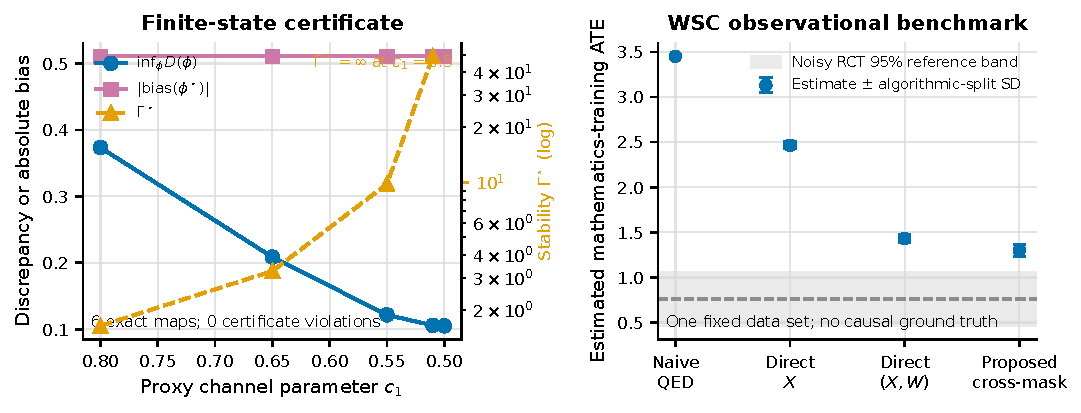
\includegraphics[width=\linewidth]{../figures/final/figure_certificate_wsc.pdf}
\caption{Certificate and observational diagnostics. Left: as the finite-state proxy channel approaches non-injectivity, the observable discrepancy decreases while realized bias remains fixed and the required stability constant diverges. Right: WSC estimates relative to the noisy randomized reference. Error bars for fitted WSC methods are standard deviations across ten algorithmic splits of one fixed data set, not Monte Carlo uncertainty. The WSC panel has no causal ground truth and reports only the unconstrained cross-mask learner as the proposed method.}
\label{fig:certificate-wsc}
\end{figure}

\clearpage
